\chapter{Supporting Materials}

This would be any supporting material not central to the dissertation.

\begin{itemize}
\item Choice of $\epsilon$ in Numerical QPI Simulations;
\item diagrams of specialized equipment developed.;
\item copies of questionnaires and survey instruments.
\end{itemize}

\chapter{Major repair of Createc STM during 2023-2024}\label{appen:fix}

\chapter{Non-Intrinsic Defects in PtSn\textsubscript{4}} \label{appen:non-intrinsic}


%todo: make differentiation between the non/intrinsic defect type and non/intrinsic defect number. meaning that there could be a defect type with both intrinsic and non-intrinsic origin, e.g 20% being intrinsic but 80% extrinsic.
\par In our experiment, we have observed that the Sn1 defect, located at the Sn-site, is highly mobile under conditions of high scanning biases (exceeding 600mV). Notably, rotation of this defect is consistently observed in consecutive scans, example given in \ref{fig:Ch4_rotationcroissant}, and instances of annihilation between two Sn1 defects have also been documented, as shown in \ref{fig:Ch4_croissantannihilation} and \ref{fig:Ch4_rotationcroissant} b) to c). These events demonstrate the ability to both create and annihilate defects during scanning. This behavior also suggests that the origin of the Sn1 defect could be a Frankel pair on the Sn site. %could elaborate more on the origin of Sn1 defect. 
%todo: prepare figure on the population over different macroscopic spots. 
\par Moreover, the density of Sn1 defects varies significantly across different macroscopic locations on the crystal, as evidenced in STM observations (e.g., figure X). This variation, with density differences exceeding fiftyfold among explored locations, suggests that different cleaving planes may influence the introduction of Sn1 defects. Such spatial dependence supports the hypothesis that Sn1 defects could also be introduced during the cleaving process. 
\begin{figure}
	\centering
	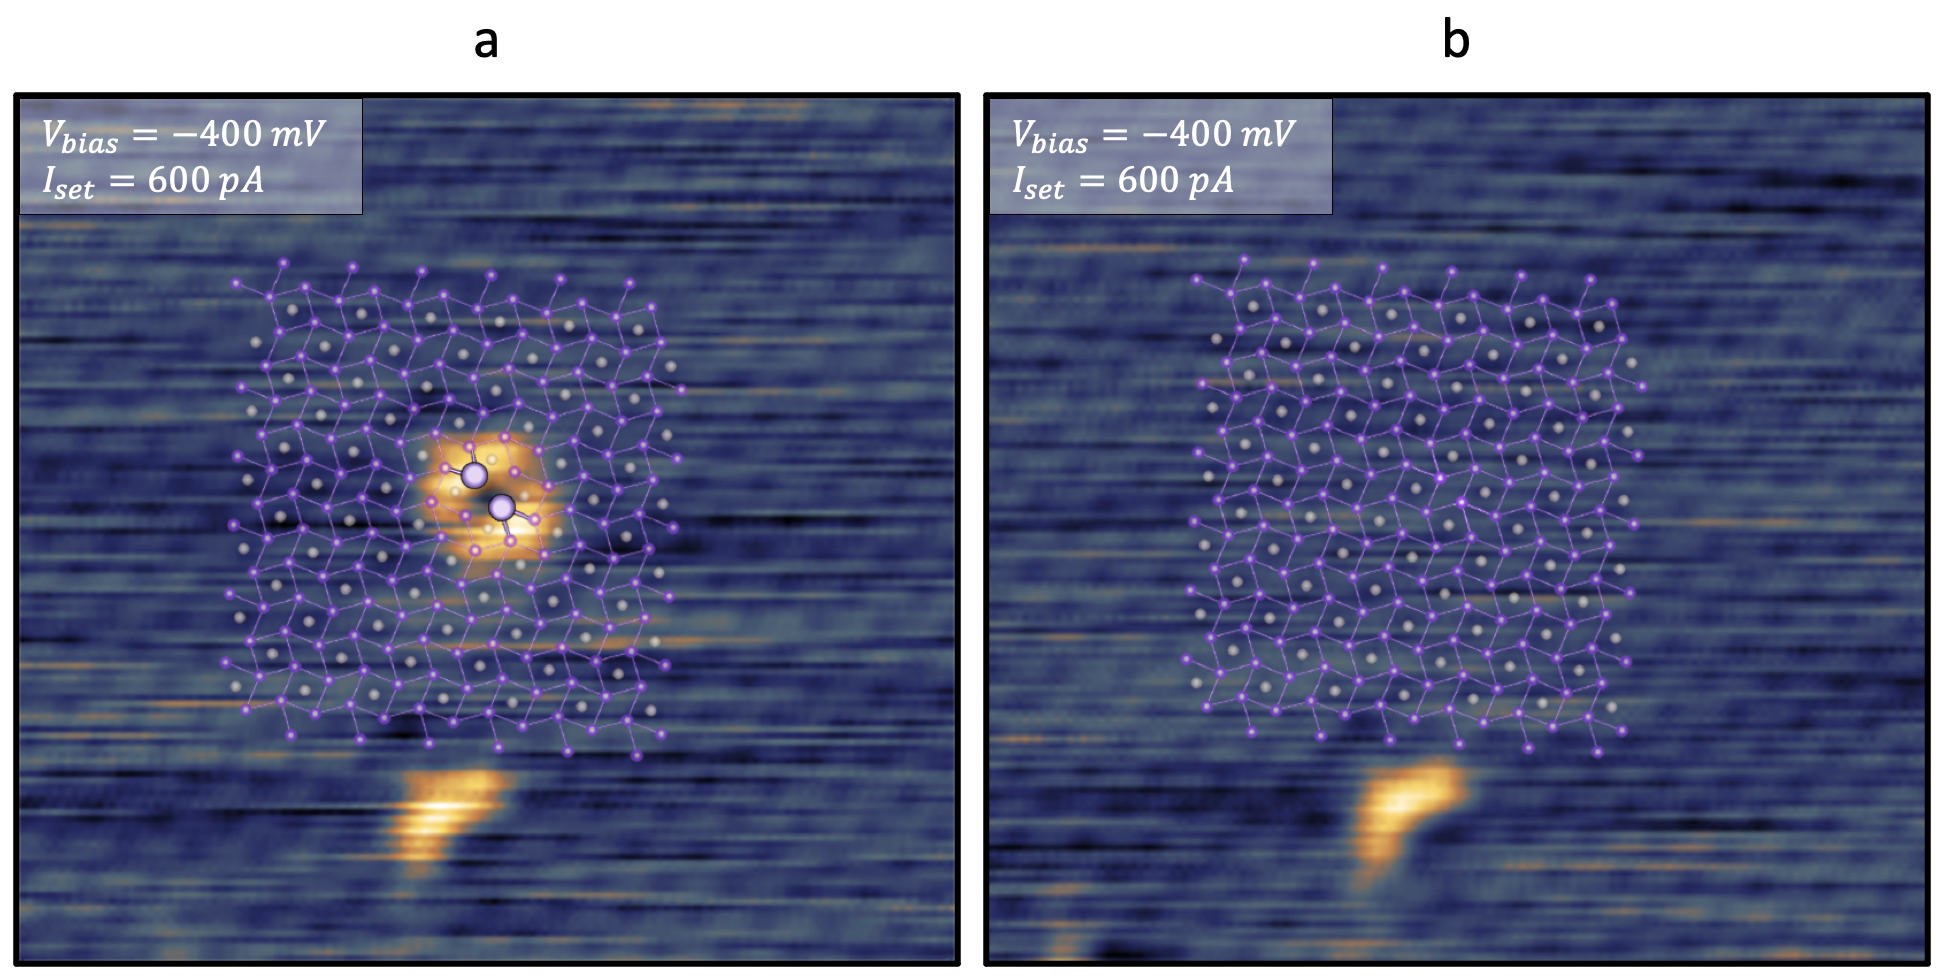
\includegraphics[width=0.8\textwidth]{Ch4_croissant.png}
	\caption{Two Sn$_1$ defect annihilation, indicating the origin of Sn$_1$ defects being from Frankel pairs}
	\label{fig:Ch4_croissantannihilation}
\end{figure}

\begin{figure}
	\centering
	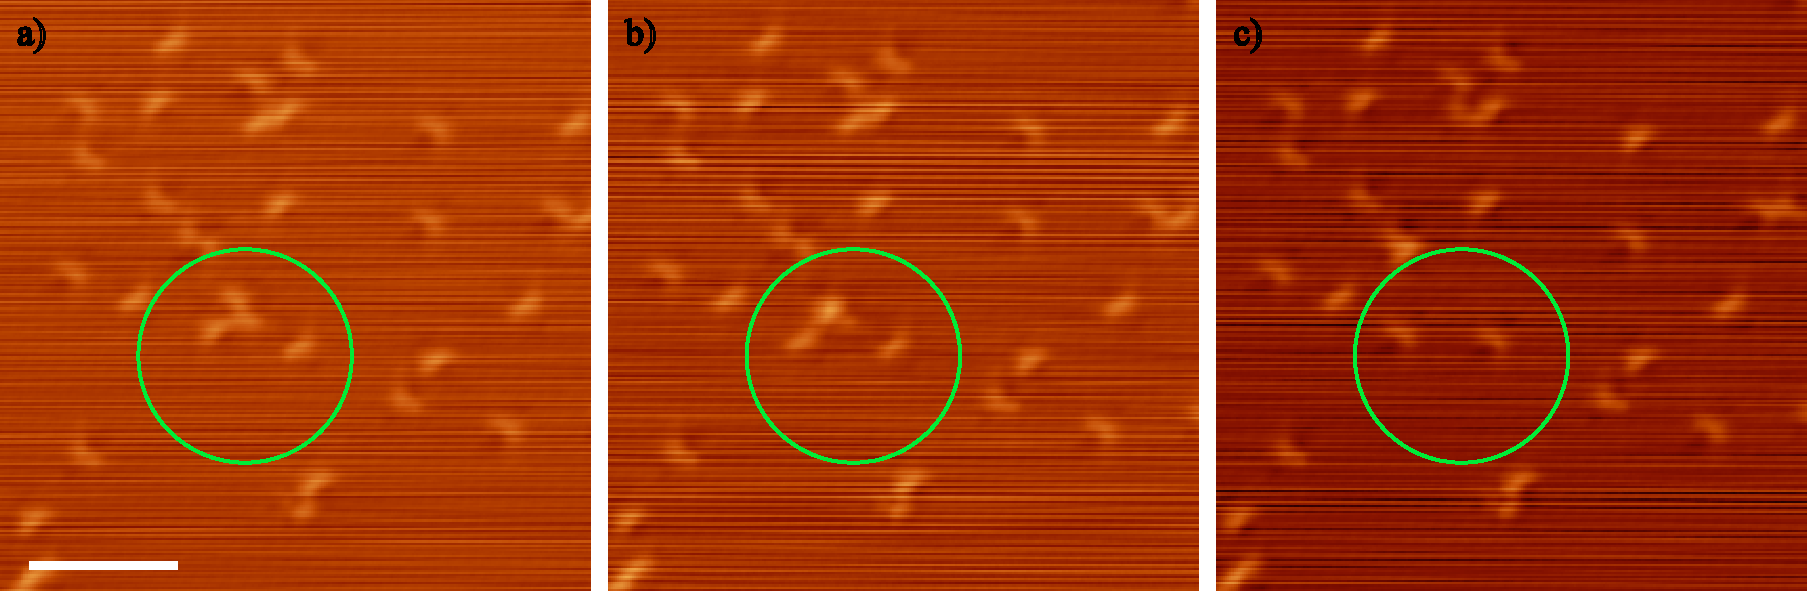
\includegraphics[width=0.8\textwidth]{Ch4_rotationcroissant.pdf}
	\caption{Sn$_1$ defect under consecutive scans, rotations and annihilation were found in the green circle.}
	\label{fig:Ch4_rotationcroissant}
\end{figure}
\par While there is no direct evidence to suggest that Sn2 and Sn3 defects are non-intrinsic, the observed decrease in their densities from samples with higher residual resistivity ratio (RRR) to those with lower RRR supports the likelihood of these defects also being non-intrinsic. This variation could be indicative of differences in crystal order influenced by experimental conditions rather than intrinsic material properties.

\par In conclusion, while the intrinsic qualities of PtSn$_4$ are well-represented in STM studies, the influence of experimental techniques such as cleaving and scanning under bias voltage introduces a variety of non-intrinsic defects. However, it is worth noting that despite the ability to introduce these defects via experimental manipulations, these defects can still intrinsically exist in bulk samples, making the studies around properties of these defects relevant. 


\chapter{Choice of $\epsilon$ in Numerical QPI Simulations} \label{app:epsilon}

In numerical simulations of quasiparticle interference (QPI) patterns on a square lattice, the parameter $\epsilon$, which enters as an $i\epsilon$ term in the Green's function, plays a pivotal role. Its selection is guided by both physical considerations and numerical stability requirements. In this appendix, we discuss the factors influencing the choice of $\epsilon$ and the trade-offs involved.

In a real material, quasiparticles have finite lifetimes due to various interactions, such as electron-electron, electron-phonon, and impurity scattering. The $i\epsilon$ term in the Green’s function is introduced as a phenomenological means to incorporate this finite lifetime. If experimental measurements or more detailed microscopic calculations suggest a particular scattering rate or linewidth, denoted by $\Gamma$, it is physically reasonable to choose $\epsilon \sim \Gamma$. For example, if the typical inverse lifetime is on the order of a few percent of the hopping parameter $t$, one might set $\epsilon \approx 0.01\,t$ to $0.05\,t$. A finite $\epsilon$ broadens sharp spectral features—such as van Hove singularities or defect-induced resonances—into Lorentzian peaks. However, if $\epsilon$ is too small, these peaks become excessively sharp, which may lead to numerical artifacts like spikes or convergence issues that do not accurately reflect the intrinsic physics. Conversely, an overly large $\epsilon$ may result in over-broadening, causing a loss of resolution in the QPI pattern.

The $i\epsilon$ prescription also has important implications for numerical stability and convergence. By moving poles away from the real axis, a finite $\epsilon$ prevents numerical divergences when evaluating the Green's function, particularly near band edges or resonances. In practice, when performing $k$-space integrations or Fourier transforms, the finite $\epsilon$ regularizes contributions from singular points, thereby enhancing the convergence of these integrals. Nevertheless, there is an inherent balance to be struck: while a smaller $\epsilon$ might capture finer spectral details, a slightly larger value is often required to ensure numerical stability. In some instances, adaptive schemes are used—starting with a larger $\epsilon$ for stability and then systematically reducing it while monitoring the convergence of the results.

Another important consideration is the relative scale of $\epsilon$ compared to other energy scales in the system. The dimensionless parameter in the Green’s function is frequently expressed as
\[
b = \frac{\omega + i\epsilon - E_0}{2t},
\]
which naturally suggests that $\epsilon$ should be small compared to the hopping parameter $t$ (and by extension, the bandwidth) so that it acts merely as a minor broadening factor rather than dominating the energy scale of the system. Additionally, in lattice simulations the momentum space is discretized, and a minimum broadening is required to mitigate aliasing or discretization errors. If $\epsilon$ is chosen too small, the computed density of states or QPI patterns may become overly sensitive to finite-size effects associated with the simulation grid.

Finally, practical considerations in QPI simulations often involve matching the simulation parameters to experimental observations. For instance, if scanning tunneling microscopy (STM) data show broadened features with a known linewidth, setting $\epsilon$ to mimic that broadening can enhance the fidelity of the simulation. It is also advisable to conduct sensitivity analyses by varying $\epsilon$ within a physically reasonable range. If the qualitative features of the QPI pattern remain robust under small changes in $\epsilon$, one can be more confident that the simulation is capturing the correct underlying physics.

In summary, the choice of $\epsilon$ in numerical QPI simulations is a balancing act. It must be small enough relative to the hopping parameter $t$ and the system's bandwidth to ensure that it only introduces a controlled broadening reflective of the finite quasiparticle lifetime, yet large enough to regularize singularities and smooth out discretization effects inherent in a finite simulation grid. By judiciously selecting $\epsilon$, one achieves both physical accuracy and numerical robustness in the simulation results.

\chapter{System parameter space of MC-SBD-STM}
this talks about how we chose the optimal parameter for synthetic dataset runs. 

\chapter{Streak detection mechanism}
